\documentclass{beamer}

\usepackage{fontspec}
\usepackage{xeCJK}
\setCJKmainfont{DFFN_R3.TTC}
\XeTeXlinebreaklocale "zh"
\XeTeXlinebreakskip = 0pt plus 1pt
\linespread{1.3}
\allowdisplaybreaks

\newcommand{\weib}{\CJKfamily{weib}}
\newcommand{\hkss}{\CJKfamily{hkss}}
\newcommand{\hksy}{\CJKfamily{hksy}}
\newcommand{\lth}{\CJKfamily{lth}}
\usepackage{color}
\usepackage{booktabs}
\usepackage{tabularx}
\usepackage{caption}
\usepackage{tikz}
\usepackage{verbatim}
\usepackage{pgfplotstable}
\pgfplotsset{width=12cm}
\pgfplotsset{height=7cm}
\pgfplotsset{compat=1.13}

\usetheme{EastLansing}
\usetikzlibrary{positioning}
\useinnertheme{rectangles}
\usefonttheme{professionalfonts}

\newcommand{\lw}{0.8mm}
\setbeamercovered{transparent}


%\AtBeginSection[]
%{
  %\begin{frame}<beamer>
	%\frametitle{報告大綱}
	%%\frametitle{RoadMap}
    %\tableofcontents[currentsection]
  %\end{frame}
%}

\title{Paper Introduction}
\subtitle{\textcolor[rgb]{0.00,0.50,1.00}{{Speech Processing \& Machine Learning Laboratory}}}
\author{徐瑞陽}
\date{2019/06/12}
\begin{document}

\begin{frame}
\maketitle
\end{frame}

\begin{frame}
\frametitle{Outline}
\tableofcontents
\end{frame}


\section{Transferring Knowledge Across Learning Process}
\begin{frame}
  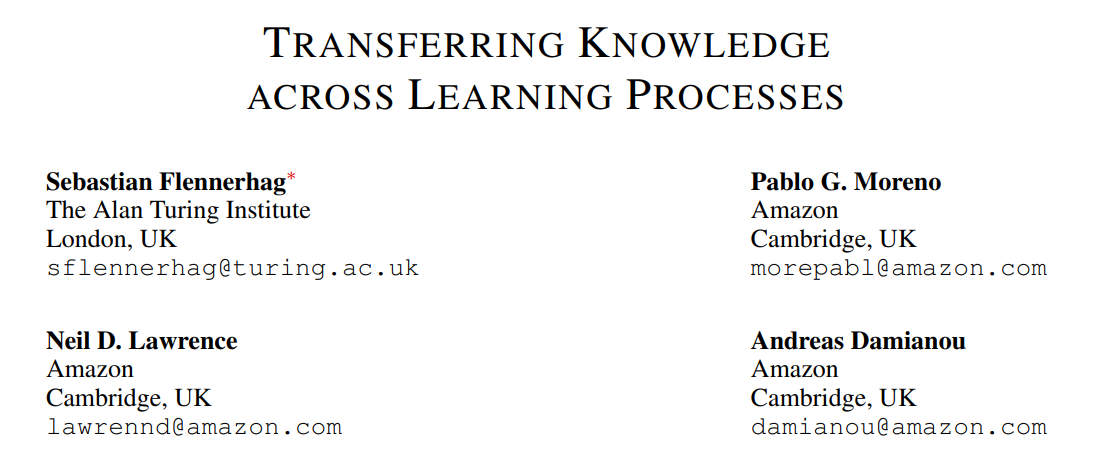
\includegraphics[width=\textwidth]{fig/p1-title.png}
  \center ICLR 2019
  \center (6,8,8)
\end{frame}

\begin{frame}{Motivation}
  Current meta-learning algorithm mainly focus on \textbf{few-shot learning} problem. 
  \begin{itemize}
    \item Few samples for each task
    \item Few gradient steps (to avoid overfitting)
  \end{itemize}
\end{frame}

\begin{frame}{Motivation}
  Can we extend meta-learning to more complex task?
  \begin{itemize}
    \item \textbf{low-resource} rather than \textbf{few-shot}
    \item \textbf{rapid adaptation} (e.g thousands of gradient steps) rather than \textbf{few} gradient steps
  \end{itemize}
\end{frame}

\begin{frame}{Highlight}
  \begin{itemize}
    \item New meta-objective (to meta-learn better \textbf{initial weights})
    \item More realistic experiment settings
  \end{itemize}
\end{frame}

\begin{frame}{New Meta-objective}
  \begin{itemize}
    \item The length of learning process is small
    \item The learning process is smooth
  \end{itemize}

\end{frame}

\begin{frame}{New Meta-objective}
  Minimize the travelling length in a task manifold $M$

  \begin{itemize}
    \item $p = (\theta,f(\theta)) \in M$
    \item $f(\cdot)$: objective function
  \end{itemize}
  \center 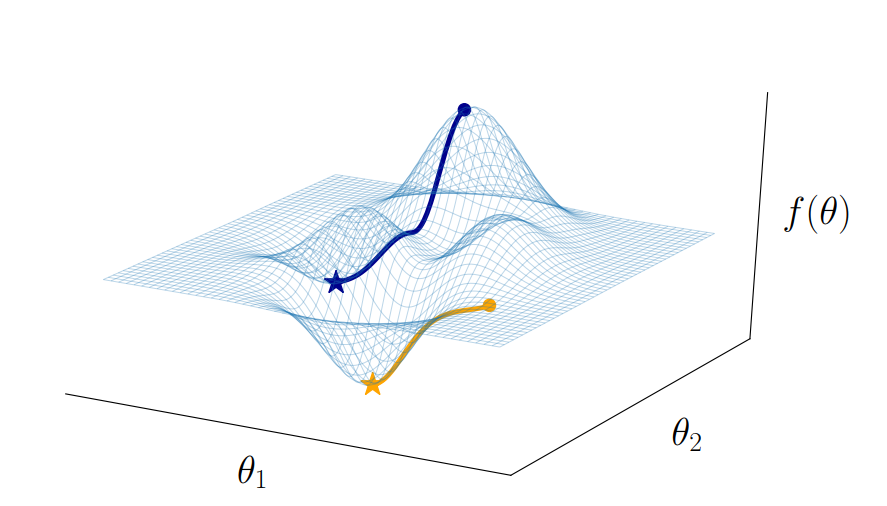
\includegraphics[width=0.7 \textwidth]{fig/p1-manifold.png}
\end{frame}

\begin{frame}{Idea}
\center 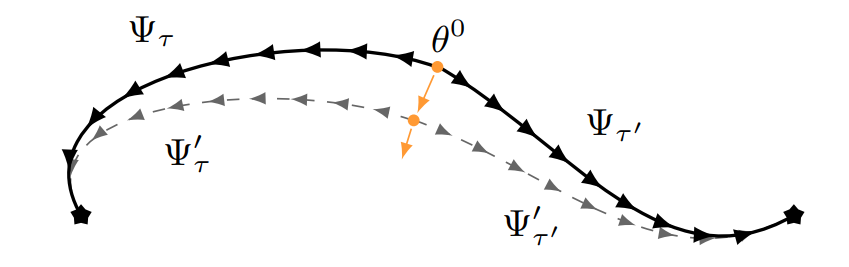
\includegraphics[width = \textwidth]{fig/p1-idea.png}
\end{frame}


\begin{frame}{Some Notation about Learning Process}
  \begin{itemize}
    \item learning process $\gamma$ is a curve on $M$
    \item $\gamma^i$ is the $i$-th point on $\gamma$ (discrete version)
    \item distance metric $d(\theta^0;M) = \sum_{i=0}^{K-1} ||\gamma^{i+1} - \gamma^i||_2$
  \end{itemize}
\end{frame}

\begin{frame}
  \begin{block}{Meta Objective}
  \[
    \theta^{\star} = \arg\min_{\theta^0} F(\theta^0) = \mathbb{E}_{\tau \sim p(\tau)} [\, d(\theta^0;M_\tau) ]\,
  \]
  \end{block}

  \begin{itemize}
    \item $\theta_{\tau}^{i+1} = u_\tau(\theta^i_\tau), \quad \theta_\tau^0 = \theta^0 \, \text{is shared across tasks}$
    \item $\theta^0 \in \Theta = \cap_\tau \lbrace \theta^0 | f_\tau(\theta_\tau^{K_\tau}) \leq f_\tau(\psi_\tau^{K_\tau}) \rbrace$
    \item $\psi_\tau^0$ can be random initialization or pretrained weights
  \end{itemize}
\end{frame}

\begin{frame}{After...}
  \begin{itemize}
    \item Combine second constraint into distance metric
    \item Approximate Jacobian matrix of $\theta^0$ as Identity matrix
    \item The new derived initial weight $\theta^0$ will used as $\psi_\tau^0$ in the following iteration
    \item And some approximations...
  \end{itemize}
\end{frame}

\begin{frame}{Meta Gradient}
  \[
    \nabla F(\theta^0) = \mathbb{E}_{\tau \sim p(\tau)} \Big [\, \sum_{i=0}^{K_\tau - 1} (\Delta f_\tau^i \nabla f_\tau(\theta_\tau^i) + \Delta \theta_\tau^i ) \Big]\,
  \]

  Comparison:
  \begin{itemize}
    \item FOMAML: $\mathbb{E}_{\tau \sim p(\tau)} \Big [\, \nabla f_\tau(\theta^{K_\tau -1}_\tau) \Big ]\,$ 
    \item Reptile: $\mathbb{E}_{\tau \sim p(\tau)} \Big [\, \sum_{i=0}^{K_\tau - 1} \Delta \theta_\tau^i \Big ]\,$
  \end{itemize}
\end{frame}

\begin{frame}{Experiment on Multi-CV}
  Consider set of CV datasets as distinct tasks (Face, MNIST, NotMNIST, Cifar10, Traffic Sign, SVHN...), then pretrain on all but one held-out task.\\ 
  $\quad$\\ 
  In meta-training, we train on each task for one epoch.\\
  The following value in the table means error rate.
\end{frame}

\begin{frame}{Experiment on Multi-CV}
  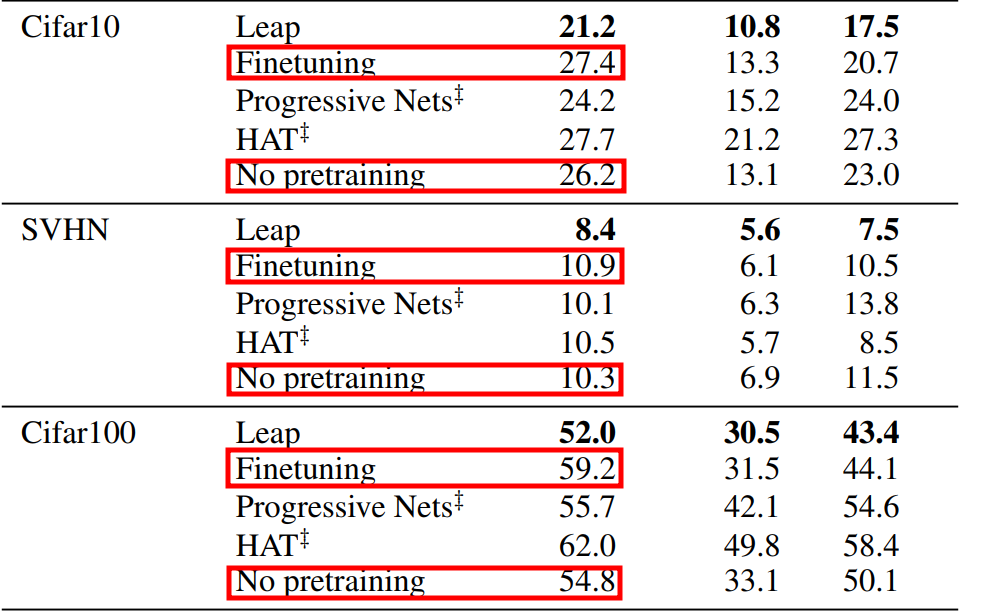
\includegraphics[width=\textwidth]{fig/p1-MultiCV.png}
\end{frame}

\begin{frame}{Observation - Finetuning is worse than no-pretraining?}
  Pretraining on all other tasks available sometimes are not good

  \begin{itemize}
    \item Need to solve both new task and retain high performance on previous tasks (the latter acted as \textbf{regularization})
    \item A single model encode both task-generic and task-specific information,
      it must either saturate or grow in size
  \end{itemize}
\end{frame}

\begin{frame}{Some Thoughts}
  \begin{itemize}
    \item Large-scale meta-learning mentioned in this paper is more suitable for speech-related applications(e.g ASR, TTS)
    \item If we still want to use fine-tuning to improve performance under low-resource scenerio, which source tasks we should choose? 
  \end{itemize}
\end{frame}

\section{Massively Multilingual Adversarial Speech Recognition}
\begin{frame}
  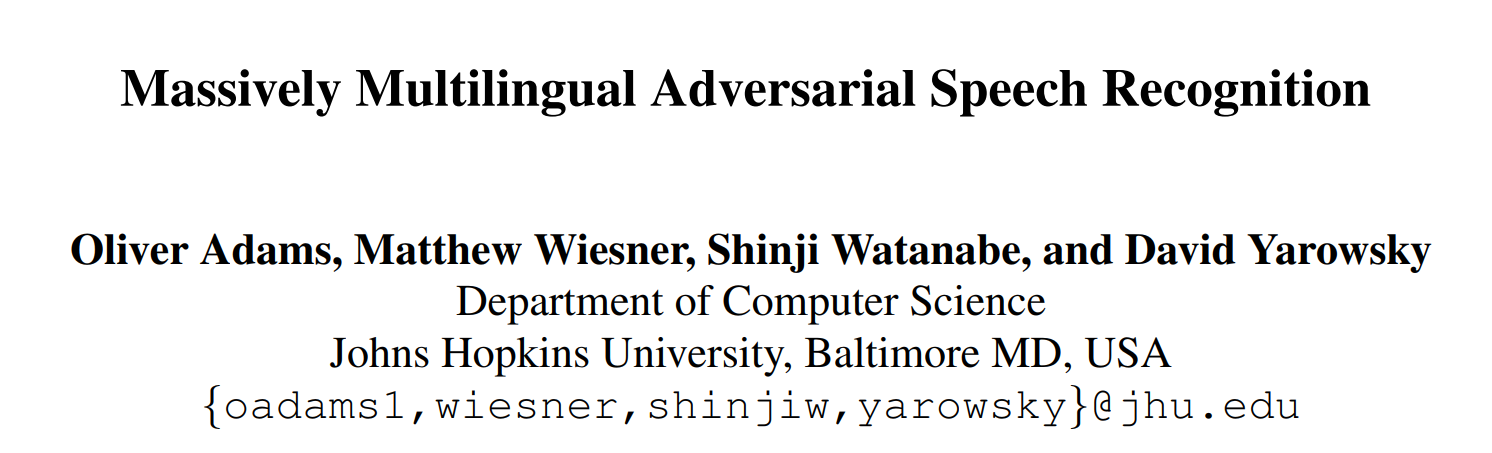
\includegraphics[width=\textwidth]{fig/p2-title.png}
  \center NAACL 2019
\end{frame}

\begin{frame}{In Brief}
  Pretraining on multilingual corpus as initial weight, then adapt to target languages (which usually low-resource), and to see which criteria is important selecting pretraining languages
\end{frame}

\begin{frame}{Highlight}
  \begin{itemize}
    \item Pretrained corpus contain \textbf{100} languages
    \item Experiment and analyze relative importance of similarity between pretraining and target languages
    \item \textit{(not so novel)} Both grapheme and phoneme objective
    \item \textit{(not so novel)} Language-adversarial pretraining
  \end{itemize}
\end{frame}

\begin{frame}{Model Architecture}
  \center 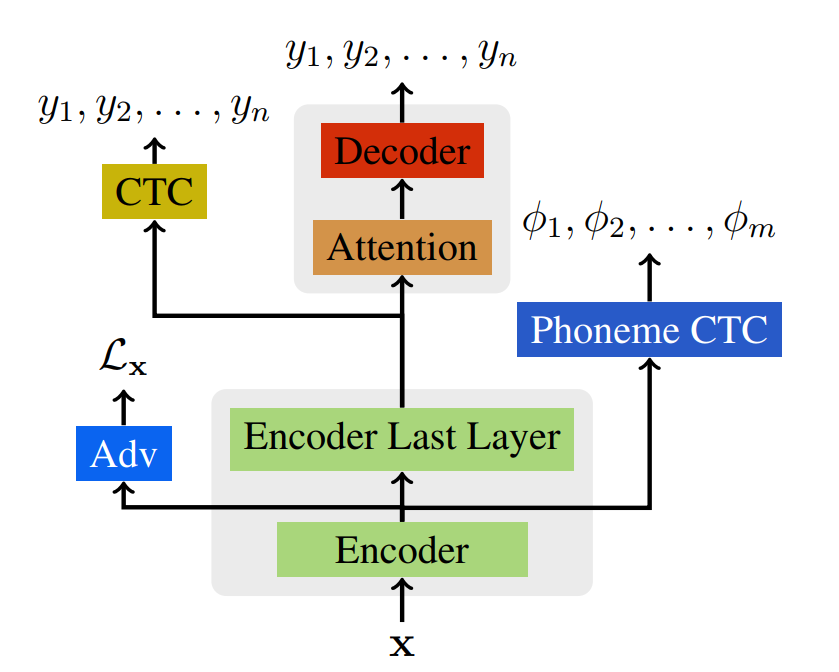
\includegraphics[width=0.6\textwidth]{fig/p2-arch.png}
\end{frame}

\begin{frame}{Experiment}
  Corpus: CMU Wilderness (ICASSP 2019, from CMU)
  \begin{itemize}
    \item Reading of Bible (with BGM), SR: 16kHz
    \item Over \textbf{700} languages
    \item Each contains around 20 hours sentence-lengthed audio with transcriptions
  \end{itemize}
  Setting
  \begin{itemize}
    \item Reading Adaptation: adapt to target languages and target speakers
    \item Language Adaptation: adapt to target languages but \textbf{non-target} speakers\\
      (Focus on this in the following discussion)
  \end{itemize}
  %The difference is, when fine-tuning, whether we can use that speaker's reading as training data
\end{frame}

\begin{frame}{Features of Languages}
  \begin{itemize}
    \item Phonological feature vectors (from PHOIBLE)
    \item Geography: location on Earth
  \end{itemize}
\end{frame}

\begin{frame}{Experiment}
  \center 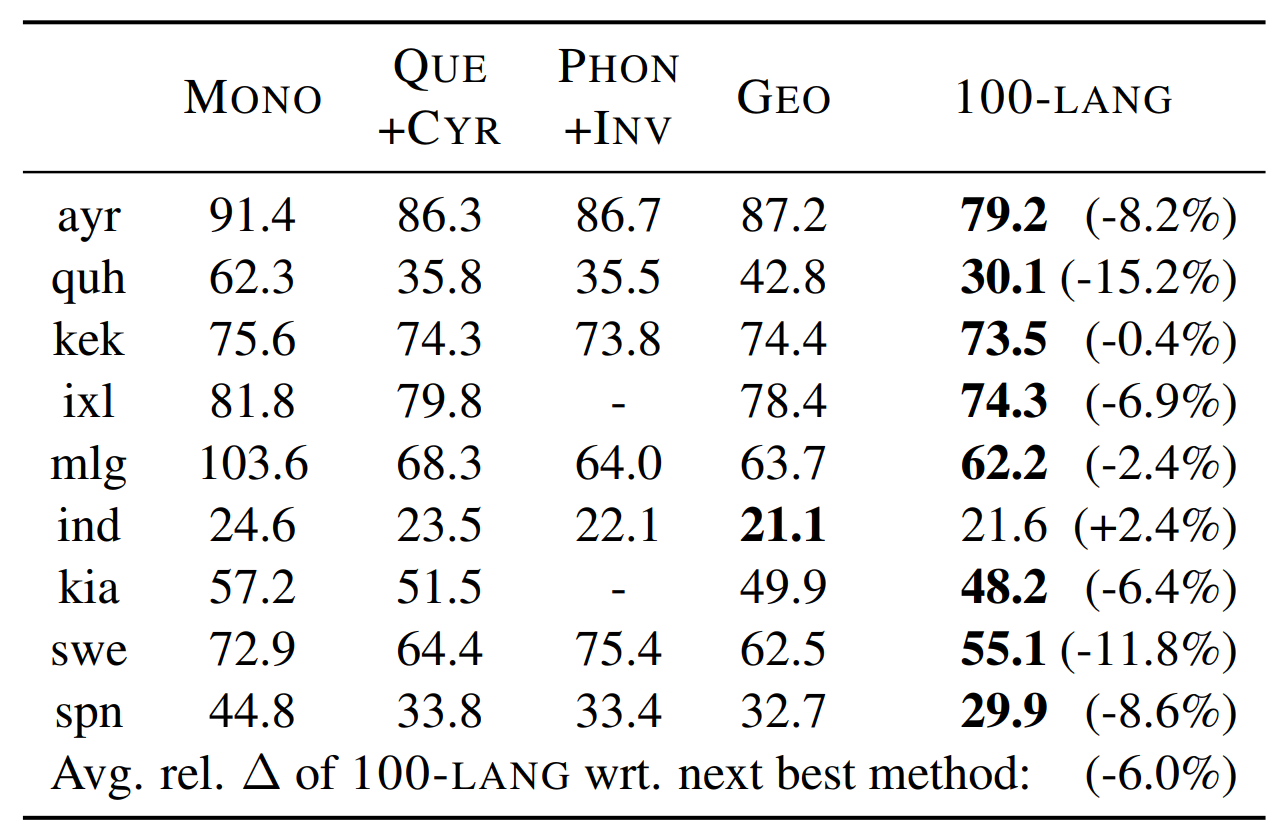
\includegraphics[width=0.6\textwidth]{fig/p2-result.png}

  \begin{itemize}
    \item PHON, GEO: pretrained on top 7/14 languages which are PHON/GEO-similar
    \item 100-LANG: pretrained on all available languages ($\approx$ 1650 hrs)
  \end{itemize}
\end{frame}

\begin{frame}{Conclusion}
  \begin{itemize}
    \item Exposure to more speech in pretraining is the most important thing\\
      (should minimize the mismatch to unseen speaker)

      \item BTW, CMU Wilderness is not available at the moment... 0w0
  \end{itemize}
\end{frame}


\section{Hierarchically Structured Meta-learning}
\begin{frame}
  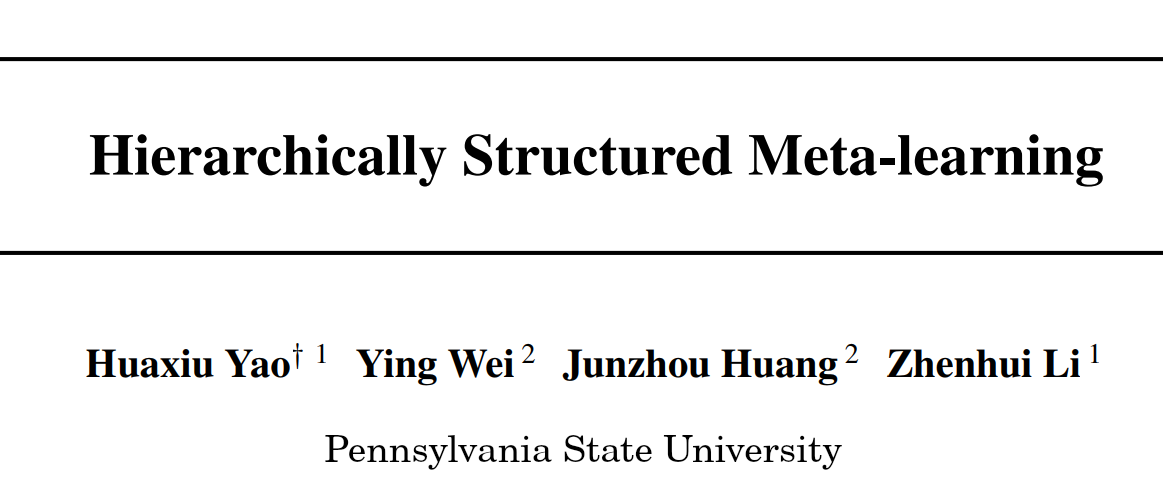
\includegraphics[width=\textwidth]{fig/p3-title.png}
  \center ICML 2019
\end{frame}

\begin{frame}{Motivation}
  \begin{itemize}
    \item Current meta-learning assume the transferable knowledge is globally shared
  \end{itemize}
    \center 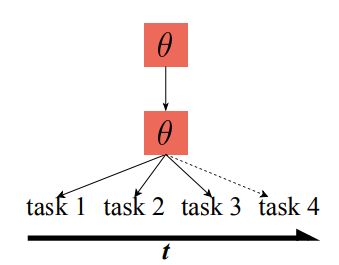
\includegraphics[width=0.4\textwidth]{fig/p3-global.png}

  Note: This paper meta-learns \textbf{initial weights} (like MAML)
\end{frame}

\begin{frame}{Proposed Framework}
  \begin{itemize}
    \item Learn the knowledge within the cluster (rather than global)
    \item Initiate a new cluster if the task is too different from existing clusters
  \end{itemize}
    \center 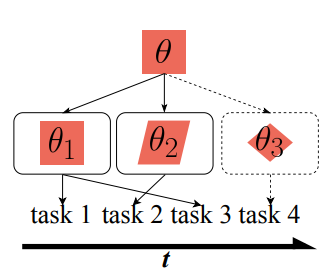
\includegraphics[width=0.4\textwidth]{fig/p3-specific.png}
\end{frame}

\begin{frame}{Proposed Framework}
    \center 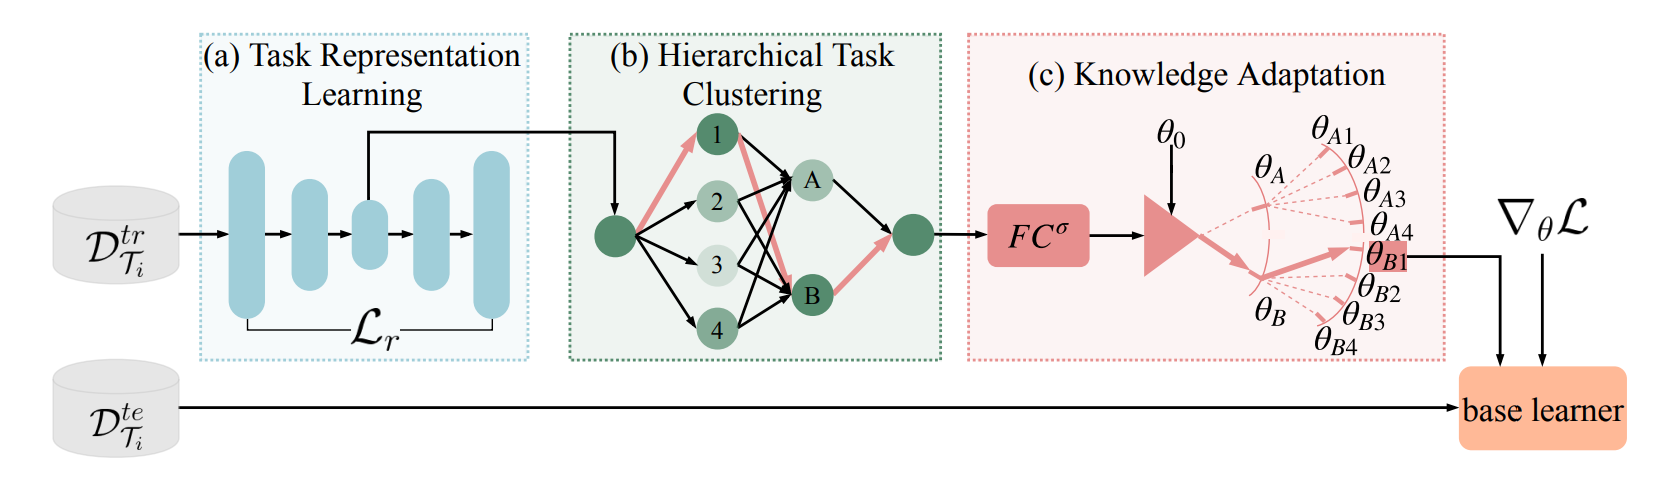
\includegraphics[width=\textwidth]{fig/p3-arch.png}
\end{frame}

\begin{frame}{Proposed Framework}
  \begin{itemize}
    \item \textbf{Task Representation} to extract feature of task $i$ :\\ \textit{Recurrent Autoencoder} Aggregator $\rightarrow$ get $\mathbf{g}_i$
    \item \textbf{Hierarchical Task Clustering} to locate the task belongs to:\\ soft assignment $\rightarrow$ get final representation $\mathbf{h}_i^L$ 
    \item \textbf{Knowledge Adaptation} to combine global and cluster-specific info: \\
      \begin{itemize}
        \item global info: $\theta_0$
        \item cluster-specific gate: $\mathbf{o}_i = \texttt{FC}(\texttt{concat}(\mathbf{g}_i,\mathbf{h}_i^L))$
      \end{itemize}
  \end{itemize}
  \center $\Rightarrow$ cluster-specific initial weight: $\theta_{0,i} = \theta_0 \circ \mathbf{o}_i$
\end{frame}


\section{MISC}
\begin{frame}
	\begin{center}
    %\weib{\LARGE{謝謝聆聽!}}
    \LARGE{Questions?}
	\end{center}
\end{frame}


\subsection{Appendix}
\end{document} 
